\gr
\chapter{Καρδιακές αρρυθμίες}
Στο προηγούμενο κεφάλαιο παρουσιάστηκε η ανατομία και η βασική λειτουργία της ανθρώπινης καρδιάς, ο καρδιακός ρυθμός (Σχήμα 2.1), η απεικόνισή του και η ερμηνεία του μέσω του ΗΚΓ (Σχήμα 2.2). Μέσω αυτού του εργαλείου είναι εφικτή η διάγνωση και η πρόληψη ποικίλων καρδιακών δυσλειτουργιών. Όταν οι δυσλειτουργίες αυτές δεν οφείλονται σε θόρυβο από το εξωτερικό περιβάλλον και το ΗΚΓ, προέρχονται από έναν καρδιακό ρυθμό που αποκλίνει του φυσιολογικού. Οι καταστάσεις αυτές ονομάζονται αρρυθμίες και θα αναλυθούν στο τρέχον κεφάλαιο. Πιο συγκεκριμένα, θα παρουσιαστεί ο ακριβής ορισμός της αρρυθμίας, ποια διαμερίσματα της καρδιάς αντιστοιχούν σε ποιες κατηγορίες αρρυθμιών, πώς αποτυπώνονται στο καρδιογράφημα, αλλά και με ποιες μεθόδους υπολογίζονται. \par
%\section{Ορισμός}
Ο όρος αρρυθμία καλύπτει ένα ευρύ φάσμα καρδιακών φαινομένων και αναταραχών. Ως καρδιακή αρρυθμία ορίζεται η απόκλιση από το φυσιολογικό παλμό. Κατά τη διάρκεια των αρρυθμιών ο παλμός της καρδιάς μπορεί να είναι πολύ χαμηλός, πολύ υψηλός ή εντελώς ακανόνιστος. 
\par
Όπως σχολιάστηκε στο προηγούμενο κεφάλαιο, ένας φυσιολογικός παλμός παράγεται από το φλεβόκομβο (\en SA node \gr) και στη συνέχεια επιβραδύνεται καθώς περνά από τον κολποκοιλιακό κόμβο (\en AV node\gr ). Έπειτα, περνά στα τέσσερα κύρια διαμερίσματα της καρδιάς, τους κόλπους και τις κοιλίες και τέλος σε όλα τα διαφορετικά σημεία του σώματος. Οποιαδήποτε κατάσταση αποκλίνει από αυτή θεωρείται αρρυθμία.
\par
Οι αρρυθμίες χωρίζονται σε δύο μεγάλες κατηγορίες: τις βραδυκαρδίες, δηλαδή καταστάσεις στις οποίες ο καρδιακός παλμός είναι χαμηλότερος του κανονικού μέσου όρου (60 παλμοί το λεπτό) και τις ταχυκαρδίες, καταστάσεις στις οποίες ο καρδιακός παλμός αυξάνεται σε σημείο άνω του φυσιολογικού ανθρώπινου (100 παλμοί το λεπτό). Ειδικότερα, οι αρρυθμίες χωρίζονται με βάση το σημείο προέλευσης, τον τρόπο μετάδοσης και τις ασθένειες με τις οποίες συσχετίζονται. Οι αρρυθμίες μπορεί να εμφανίζονται μεμονωμένα (ένας μεμονωμένος αποκλίνων χτύπος) αλλά και σε σύνολα (δύο, τρεις ή και περισσότεροι συνεχόμενοι μη φυσιολογικοί παλμοί που αποτυπώνονται στο ΗΚΓ σε μοτίβα). 
\par
Τα άτομα που εμφανίζουν καρδιακές αρρυθμίες ενδέχεται να πάσχουν από κάποια ασθένεια ή και να είναι απόλυτα υγιή, καθώς οι αρρυθμίες σε μικρό ποσοστό, είναι απολύτως φυσιολογικές. Σε περιπτώσεις όμως, που εμφανίζονται τακτικά μπορεί να υποδείξουν κάποιο υποκείμενο νόσημα επικίνδυνο για την υγεία. Η γενική παρουσία αρρυθμιών συσχετίζεται με υψηλότερη πιθανότητα νοσηρότητας και θνησιμότητας [18]-[22], [24], [26]-[28]. 
\begin{figure}[b]
	\centering
	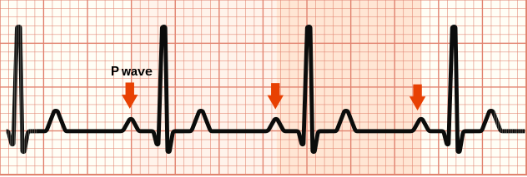
\includegraphics[scale=0.5]{normal.png}
	\caption{Φυσιολογικός καρδιακός ρυθμός \en\protect\url{https://commons.wikimedia.org/wiki/Main_Page}}
\end{figure}
\section{Κατηγοριοποίηση αρρυθμιών}
Οι αρρυθμίες μπορούν να χωριστούν στις ακόλουθες γενικές κατηγορίες:
\begin{figure}[h]
	\centering
	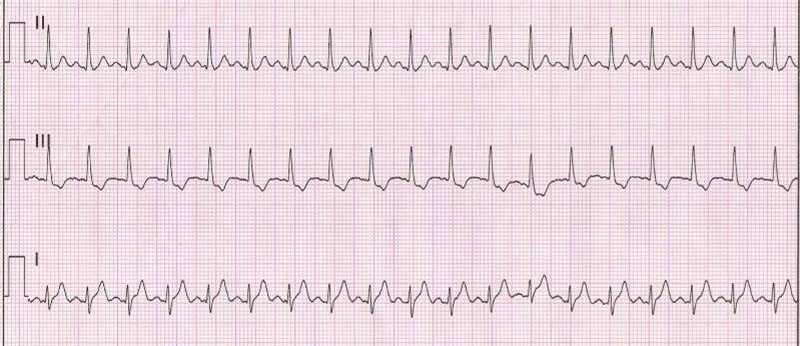
\includegraphics[scale=0.3]{Sinus_Tachycardia_Unlabeled.jpg}
	\caption{Τυπική αναπαράσταση ταχυκαρδίας σε ΗΚΓ \en\protect\url{https://en.wikipedia.org/}}
\end{figure}
\subsection{Με βάση το σημείο εκκίνησής τους στον καρδιακό μυ}
\subsubsection{Κολπική αρρυθμία} 
Υπάρχουν τέσσερις βασικές αρρυθμίες με σημείο εκκίνησης τους κόλπους της καρδιάς: φλεβοκομβική ταχυκαρδία, κολπική μαρμαρυγή, κολπικός πτερυγισμός και κολπική ταχυκαρδία. Επιπλέον στη γενικότερη κατηγορία των καρδιακών παθήσεων με σημείο εκκίνησης τους καρδιακούς κόλπους εντάσσεται και η πρόωρη κολπική σύσπαση ή έκτοπη κολπική σύσπαση (ή συστολή).
\begin{itemize}
	\item Φλεβοκομβική ταχυκαρδία (\en Sinus tachycardia \gr). Συνήθως αποτελεί φυσιολογικό γεγονός που επιδεινώνεται εξαιτίας κάποιας φαρμακευτικής αγωγής. Η μορφολογία του Ρ επάρματος επηρεάζεται με την αύξηση των παλμών και σε ακραίες περιπτώσεις δεν καταφέρνει να ξεχωρίσει από το έπαρμα Τ.  Τα αίτιά της μπορεί να είναι σωματικά, όπως ο πόνος και το άγχος, παθολογικά (παραδείγματος χάριν πυρετός), ενδοκρινολογικά (δυσλειτουργίες του θυρεοειδούς) ή φαρμακολογικά, όπως η αυξημένη αδρεναλίνη εξαιτίας κατανάλωσης καφέ και αλκοόλ. Σε πιο σπάνιες περιπτώσεις οφείλεται σε κάποιο φαινόμενο επανεισόδου του αίματος στον φλεβοκομβικό κόμβο (\en sinoatrial node re-entry \gr).  Ο καρδιακός ρυθμός φτάνει συνήθως τους 130-140 χτύπους το λεπτό.  \en [26], [42]  \gr
	\item Κολπική μαρμαρυγή \en (Atrial fibrillation). \gr Η κολπική μαρμαρυγή είναι η πιο συνήθης καρδιακή αρρυθμία και η κύρια αιτία εγκεφαλικού. Οφείλεται σε ελαττωματική ηλεκτρική δραστηριότητα στους κόλπους της καρδιάς η οποία πυροδοτεί ραγδαία παραγωγή ηλεκτρικών σημάτων και από τους δύο κόλπους. Εξαιτίας του ακανόνιστου ρυθμού το αίμα κυκλοφορεί με ασταθή και εκρηκτική ροή, κάτι που αυξάνει την πιθανότητα δημιουργίας θρόμβων που όταν μετακινηθούν στο αίμα προκαλούν τελικά εγκεφαλικό. Κατηγοριοποιείται ως ταχυαρρυθμία λόγω του αυξημένου καρδιακού ρυθμού (Σχήμα 2.3). \par
	\begin{figure}[h]
		\centering
		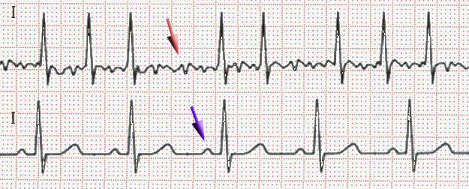
\includegraphics[scale=0.5]{Afib_ecg.jpg}
		\caption{Απεικόνιση κολπικής μαρμαρυγής \en \protect\url{https://commons.wikimedia.org/}}
	\end{figure}
	Ανάλογα με τη διάρκειά της χωρίζεται σε: παροξυσμική, κατά την οποία ο ασθενής επανέρχεται αυτόνομα σε διάστημα 7 ημερών, διαρκή ή επίμονη, στις περιπτώσεις που η μαρμαρυγή διαρκεί περισσότερο από 7 ημέρες. Σε αυτή την περίπτωση χρειάζεται εξωτερική παρέμβαση. Η κατάσταση αυτή μπορεί εν τέλει να οδηγήσει σε αναδιαμόρφωση των καρδιακών μυοκυττάρων προκαλώντας εν τέλη μυοκαρδιοπάθεια. Αυτός ο τύπος κολπικής μαρμαρυγής παρουσιάζεται τόσο ως ένα αρχικό επεισόδιο της πάθησης όσο και ως επαναλαμβανόμενο ενός περιστατικού παροξυσμικής μαρμαρυγής. Ακόμα δύο κατηγορίες είναι η: μακροχρόνια επίμονη κολπική μαρμαρυγή, όταν τα περιστατικά συμβαίνουν σε διάστημα 12 μηνών (σε αυτές τις περιπτώσεις έχει αποτύχει η φαρμακευτική αγωγή ή η όποια διαφορετική ιατρική παρέμβαση) και η μόνιμη κολπική μαρμαρυγή, περίπτωση στην οποία έχει εγκαταλειφθεί η οποιαδήποτε θεραπεία λόγω έλλειψης ανταπόκρισης του καρδιακού ρυθμού. 
	\par
	Η κολπική μαρμαρυγή χαρακτηρίζεται ως υποτροπιάζουσα όταν κάποιος ασθενής βιώνει δύο ή/και παραπάνω επεισόδια.
	\par 
	Παράγοντες αυξημένου κινδύνου για την κολπική μαρμαρυγή αποτελούν η προχωρημένη ηλικία, υποκείμενα καρδιακά νοσήματα και παθήσεις, ενδοκρινείς παθήσεις όπως ο υπερθυροειδισμός και ο διαβήτης, γενετικοί παράγοντες, νευρολογικές παθήσεις, φλεγμονές όπως η μυοκαρδίτιδα, υψηλή αρτηριακή πίεση καθώς και η υψηλή κατανάλωση αλκοόλ.
	\par
	Παρόλους τους κινδύνους που εγκυμονεί η κολπική μαρμαρυγή, έχουν αναπτυχθεί τεχνικές και θεραπείες που μειώνουν τις πιθανότητες εγκεφαλικού σε ασθενείς που πάσχουν από αυτήν. 
	Οι θεραπείες περιλαμβάνουν αντιπηκτικά φάρμακα, αγωγή για τον έλεγχο του καρδιακού ρυθμού και κάποιες παρεμβατικές διαδικασίες. [18]-[23], [29], [37], [40] 
	\begin{figure}[h]
		\centering
		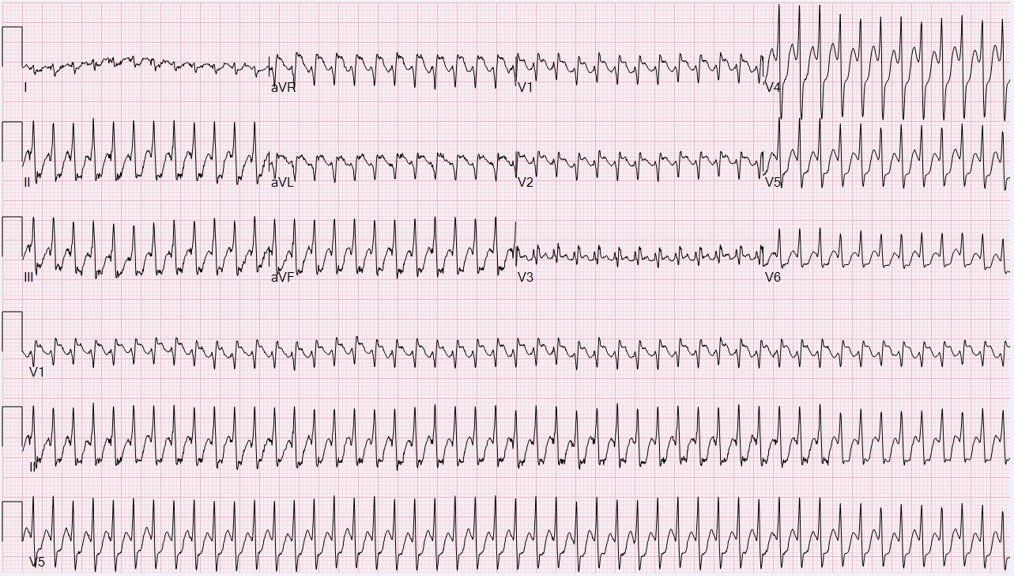
\includegraphics[scale=0.2]{Atrial_Flutter.jpg}
		\caption{Κολπικός πτερυγισμός \en\protect\url{https://commons.wikimedia.org/}}
	\end{figure}
	
	\item Κολπικός πτερυγισμός (\en Atrial flutter). \gr Ο όρος πτερυγισμός πηγάζει από μια οδοντωτή εικόνα κατά την καταγραφή του ΗΚΓ, που αντιστοιχεί σε ραγδαίο κολπικό ρυθμό, σε αντίθεση με τον ακανόνιστο ρυθμό της κολπικής μαρμαρυγής. Τα αίτια του κολπικού πτερυγισμού είναι όμοια με αυτά της κολπικής μαρμαρυγής και σε αρκετές περιπτώσεις φαινόμενα πτερυγισμού εναλλάσσονται με φαινόμενα μαρμαρυγής. Παρόλα αυτά, το 80 τοις εκατό των περιπτώσεων πτερυγισμού εμφανίζονται σε ασθενείς αρσενικού φύλου.
	\par
	Επίσης, ο πτερυγισμός χωρίζεται σε παροξυσμικό και επίμονο, ο οποίος σε πολλές περιπτώσεις χρίζει ιατρικής επέμβασης. Η απώλεια επαρκής σύσπασης των κόλπων και ο υψηλός καρδιακός ρυθμός μπορεί να οδηγήσει σε υπόταση, κυνάγχη, καρδιακή ανεπάρκεια ή συγκοπή. Σε αρκετές περιπτώσεις ο πτερυγισμός παραμένει ασυμπτωματικός για εβδομάδες και η εμμένουσα ταχυκαρδία μπορεί να καταλήξει σε καρδιακή ανεπάρκεια. Παρόλο που η κολπική λειτουργία μπορεί να επανέλθει στα φυσιολογικά επίπεδα, η αρρυθμία εμμένει και μπορεί να οδηγήσει σε αιφνίδιο θάνατο. \en [30]-[31]\gr
	\item Κολπική ταχυκαρδία \en (Atrial tachycardia). \gr Η κολπική ταχυκαρδία αφορά ηλεκτρικές ώσεις που παράγονται και παραμένουν εντός των κόλπων. Εμφανίζεται σε καταστάσεις υψηλών μεταβολικών απαιτήσεων και άγχους, όπως η υποξία, παρόλα αυτά αποτελεί καλοήθη αρρυθμία. Διαφέρει από την κολπική μαρμαρυγή και τον κολπικό πτερυγισμό και χρίζει ειδικής διάγνωσης ώστε να αποβεί σε σωστή διαχείρηση και θεραπεία. Προκαλείται από ένα ή παραπάνω μηχανισμούς που μπορούν να οδηγήσουν σε αρρυθμίες. Πολλές φορές ο μηχανισμός παραμένει απροσδιόριστος. Χωρίζεται σε τέσσερις διαφορετικές κατηγορίες: καλοήθης (εντοπίζεται συνήθως σε άτομα προχωρημένης ηλικίας. Είναι σύντομη, παροξυσμική και ο καρδιακός ρυθμός κυμαίνεται από 80 έως 140  παλμούς το λεπτό), πολυεστιακή (πολλαπλές ταυτόχρονες εκφορτίσεις του καρδιακού μυ, επηρεάζει μορφολογικά το έπαρμα Ρ και το διάστημα \en PR. \gr Συνήθως παρατηρείται σε συνδυασμό με χρόνια πνευμονική νόσο), κολπική ταχυκαρδία με αποκλεισμό (συνήθως ο κολπικός ρυθμός δεν επηρεάζεται. Αν και συνήθως αναφέρεται ως παροξυσμική, διατηρείται) και αδιάκοπη (σπάνια καρδιακή πάθηση τόσο σε παιδιά όσο και σε ενήλικες. Μοιάζει με φλεβοκομβική ταχυκαρδία και ο ρυθμός της κυμαίνεται στους 100-160 παλμούς το λεπτό). \par
	Πηγάζει συνήθως από κάποια έκτοπη σύσπαση και παράγει κολπικό ρυθμό 150-250 παλμούς το λεπτό, τα επάρματα Ρ δεν επηρεάζονται πάντα μορφολογικά. 
	Η κολπική ταχυκαρδία εμφανίζεται συνήθως σε άτομα με δομικές καρδιακές παθήσεις αλλά και ισχαιμική στεφανιαία νόσο. Ίσο βαθμό κινδύνου διατρέχουν και οι ασθενείς χωρίς δομικές νόσους και παθήσεις. Άλλα πιθανά αίτια αποτελούν οι πνευμονοπάθειες, το αλκόολ, διεγερτικά όπως οι ναρκωτικές ουσίες, η σοκολάτα και οι μεταβολικές αναταραχές. [36]-[39]  
	\begin{figure}[h]
		\centering
		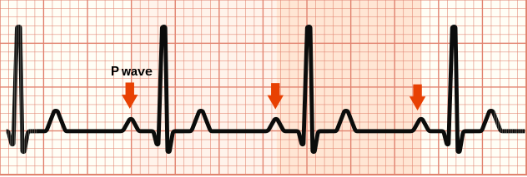
\includegraphics[scale=0.4]{normal.png}
		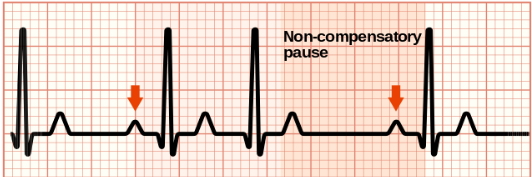
\includegraphics[scale=0.4]{pac.png}
		\caption{Εκτοπες κολπικές συσπάσεις. Στην πρώτη εικόνα (αριστερά) παρουσιάζεται ένας φυσιολογικός καρδιακός ρυθμός και στη δεύτερη (δεξιά) οι έκτοπες κολπικές συσπάσεις \en\protect\url{https://commons.wikimedia.org/}}
	\end{figure}
	\item Πρόωρη κολπική σύσπαση ή έκτακτη κολπική σύσπαση \en (Atrial premature complex or Premature Atrial Contractions - PAC). \gr  Πρόκειται για συσπάσεις που ξεκινούν από τους κόλπους αλλά δεν προέρχονται από το φλεβόκομβο, επηρεάζοντας τη μορφολογία του Ρ επάρματος. Το ρόλο του βηματοδότη αναλαμβάνει κάποιο άλλο τμήμα των κόλπων αλλά όχι ο φλεβόκομβος (μπορεί να επεμβαίνουν περισσότερα από ένα τμήματα). Συνήθως έχουν φυσιολογικό \en QRS \gr σύμπλεγμα και κανονικό, συντομότερο ή και μεγαλύτερο Ρ κύμα το οποίο είναι έκτοπο (δηλαδή συμβαίνει νωρίτερα από το φυσιολογικό). Το διάστημα \en PR \gr μπορεί να είναι ελαφρώς μεγαλύτερο. Συγκριτικά με το Ρ κύμα των φυσιολογικών συσπάσεων, το Ρ κύμα των υπερκοιλιακών αρρυθμιών διαφέρει ως προς τη μορφολογία και προηγείται χρονικά. Συνήθως ένα φυσιολογικό Ρ έπαρμα προηγείται της ενεργοποίησης των κοιλιών. Όταν το πρόωρο Ρ κύμα συμβαίνει σχετικά κοντά στο φυσιολογικό χτύπο, η μορφολογία του Ρ κύματος που παράγεται είναι ενδιάμεση του φυσιολογικού αλλά και του έκτοπου παλμού. Μπορεί να συμβαίνουν σε ζεύγη, να ακολουθούν προηγούενο \en PAC \gr, να συμβαίνουν μετά από κάθε ένα, δύο ή τρεις συνεχόμενους φυσιολογικούς παλμούς δημιουργώντας μοτίβα. Αν συμβούν αρκετά πρόωρα, μπορεί να προκαλέσουν τη δημιουργία ενός πιο πεπλατυσμένου \en QRS \gr συμπλέγματος. Οι αιτίες εμφάνισής τους μπορεί να συνδέονται με τη δομή της καρδιάς (υπερτροφική καρδιομυοπάθεια) είτε με χημικούς παράγοντες (αγωνιστές των β-υποδοχέων). Οι λόγοι που τις πυροδοτούν είναι ιδιοπαθείς, δηλαδή ποικίλοι, συχνά εμφανίζονται αυθόρμητα και η αιτία τους παραμένει άγνωστη. Οι ιδιοπαθείς πρόωρες κολπικές συσπάσεις συχνά ξεκινούν από πνευμονικές φλέβες όταν δεν υπάρχει κάποια δομική καρδιακή πάθηση. Οι αιτίες πρόκλησής τους μπορούν να ερμηνευθούν ως δομικές, χημικές ή κάποιο αποτέλεσμα διαφορετικού συνόλου καταστάσεων ή παθήσεων. Αν οι κόλποι αδυνατούν να προκαλέσουν σύσπαση, ο παλμός σταματά (δεν μπορεί να αντληθεί αίμα). Όταν υπάρχουν τρεις ή περισσότερες έκτακτες κολπικές συστολές το σήμα ερμηνεύεται ως κολπική ταχυκαρδία.
	\par
	Εντοπίζονται τόσο σε νέους ασθενείς όσο και σε γηραιότερους. Οι δομικές αιτίες τους συμπεριλαμβάνουν παθήσεις όπως η στεφανιαία νόσος, η υπερτροφική μυοκαρδιοπάθεια, τα ανευρύσματα του αριστερού κόλπου, η υπερτροφία της αριστερής κοιλίας αλλά και συγγενείς καρδιακές δυσπλασίες. Συγγενή συμπτώματα έχουν εμφανιστεί ακόμα και σε βρέφη και συνήθως τα αίτια θεωρούνται παθολογικά. Παρόλα αυτά η ανίχνευσή και ο εντοπισμός τους είναι πιο πιθανό να συμβούν κατά συνεχή καταγραφή με κάποιον καταγραφέα \en Holter \gr από ότι κατά την καταγραφή ενός ΗΚΓ. Οι επιλοκές, τέλος, που μπορούν να προκαλέσουν οφείλονται στους παράγοντες που ευθύνονται για την εμφάνισή τους. Μερικά παραδείγματα επιπλοκών είναι η κολπική μαρμαρυγή και τα ισχαιμικά εγκεφαλικά επεισόδια. Μεμονωμένες συσπάσεις δε συμβάλλουν σε αυξημένες πιθανότητες καρδιακών επεισοδίων και θανάτου. [27], [36], [37] \en
\end{itemize}
\begin{figure}[h]
	\centering
	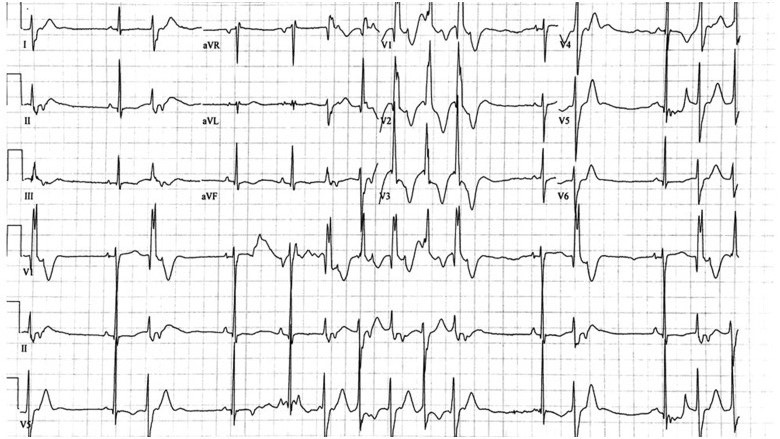
\includegraphics[scale=0.3]{ventricular tachycardia.jpg}
	\caption{Κοιλιακή ταχυκαρδία \en\protect\url{https://en.wikipedia.org/}}
\end{figure}
\subsubsection{Κοιλιακή αρρυθμία} 
Οι κοιλιακές ταχυκαρδίες αποτελούν ταχυπαλμίες που ξεκινούν στις κοιλίες της καρδιάς και είναι εξαιρετικά επικίνδυνες (110-250 χτύποι το λεπτό). Το \en QRS \gr σύμπλεγμα διαρκεί σημαντικά μεγαλύτερο διάστημα και ποικίλει σε μορφολογία. Μερικοί από τους πιθανούς τύπους εμφάνισης αποτελούν: δύο διαφορετικοί τύποι \en QRS \gr συμπλέγματος που εναλλάσσονται μεταξύ τους, περισσότεροι από δύο τύποι \en QRS \gr που εμφανίζονται στο καρδιογράφημα ή σταδιακή εναλλαγή των \en QRS \gr συμπλεγμάτων σε σχήμα και διάρκεια από μη φυσιολογικό σε φυσιολογικό. Ανάλογα με το χρονικό σημείο του παλμού κατά το οποίο εμφανίζονται, το αποτέλεσμα ποικίλει από κοιλιακή μαρμαρυγή (μη συγχρονισμένη σύσπαση διαφορετικών τμημάτων της καρδιάς), ταχυκαρδία (τρεις ή περισσότερες συνεχόμενες συστολές) ή κοιλιακό πτερυγισμό (παρουσιάζοντας μια πριονωτή εικόνα) διαταραχές οι οποίες μπορεί να αποβούν θανατηφόρα. Η στεφανιαία νόσος, το έμφραγμα του μυοκαρδίου, η αποδυνάμωση του καρδιακού μυ και άλλες παθήσεις μπορεί να προκαλέσουν κοιλιακές αρρυθμίες. H προέλευσή της βρίσκεται χαμηλότερα του κολποκοιλιακού κόμβου.
\begin{itemize}
	\item  Έκτακτη κοιλιακή συστολή, \en Premature Ventricular Contractions (PVC)\gr : Αποτελεί πρόωρη εκπόλωση του μυοκαρδίου που ξεκινά από τις κοιλίες και δημιουργεί μια επιπλέον (μη φυσιολογική) σύσπασή τους. Χαρακτηρίζονται από πρώιμο \en QRS \gr σύμπλεγμα με ανώμαλη μορφολογία και χρονική διάρκεια μεγαλύτερη των 120 \en msec \gr . Ανάλογα με ποιο τμήμα των κοιλιών συσπάται δημιουργείται και ένα διαφορετικό (μη φυσιολογικό) \en QRS \gr σύμπλεγμα. Ακολουθούνται από ένα εκτενές Τ κύμα χωρίς την ύπαρξη προηγούμενων (έκτοπων) Ρ κυμάτων και η μορφολογία των τελευταίων παραμένει ίδια. Εμφανίζονται οποιαδήποτε στιγμή του καρδιακού κύκλου και παρατηρούνται μεμονωμένα, σε ζεύγη ή έπειτα από κάθε ένα, δύο, τρεις ή και τέσσερις φυσιολογικούς παλμούς (δημιουργώντας διαφορετικά μοτίβα). Σε πολλές περιπτώσεις εμφανίζονται σε συνδυασμό με δομικές καρδιακές παθήσεις, ωστόσο παρατηρούνται και ανεξάρτητα από αυτές. 
	\par
	Κατά τη διάρκεια μιας έκτοπης κοιλιακής συστολής ο παλμός ξεκινάει από τις ίνες \en Purkinje \gr (κύτταρα υπέυθυνα για δημιουργία ηλεκτρικών ώσεων) αντί για το φλεβόκομβο. Οι πρόωρες κοιλιακές συστολές προηγούνται ενός φυσιολογικού παλμού και ο επόμενος φυσιολογικός παλμός φαίνεται να καθυστερεί, καθώς συμβαίνει μετά από μια παύση. Επιπλεόν, οι συστολές αυτές μπορούν να εμφανιστού μεμονωμένα αλλά και σε μοτίβα των δύο ή τριών συνεχόμενων παλμών· περισσότερες από τρεις συνεχόμενες συστολές αυτού του τύπου κατηγοριοποιούνται ως κολπική ταχυκαρδία.
	\par
	Στην περίπτωση που αυτού του τύπου παλμοί εναλλάσσονται συνεχώς με φυσιολογικό παλμό, ο ασθενής βρίσκεται σε κατάσταση διδυμίας \en (bigeminy).\gr Ομοίως όταν ένας φυσιολογικός παλμός μεσολαβεί μετά από δύο έκτοπες κοιλιακές συστολές ο ασθενής βρίσκεται σε τριδυμία \en (trigeminy).\gr  Όταν ανιχνεύεται στο ΗΚΓ η ύπαρξη τριών ή περισσότερων συνεχόμενων συστολών, η διάγνωση συνήθως είναι κοιλιακή ταχυκαρδία. Περαιτέρω, η αρρυθμία θεωρείται παρατεταμένη αν διαρκεί πάνω από τριάντα δευτερόλεπτα και μη παρατεταμένη στην αντίθετη περίπτωση.
	\par 
	Η πλειοψηφία αυτών των συστολών συμβαίνουν αυθόρμητα και οι αιτίες προέλευσής τους δεν είναι γνωστές. Καταστάσεις και παράγοντες που μπορεί να εντείνουν την κατάσταση είναι η ακατάσχετη κατανάλωση καφεΐνης, τα υψηλά επίπεδα στρες, η κατανάλωση αλκοόλ, ναρκωτικών ουσιών και καπνού και η έλλειψη ύπνου. Γίνονται αντιληπτές με την αίσθηση έντονων παλμών στο στήθος των ασθενών αλλά στις περισσότερες περιπτώσεις είναι καλοήθεις και δε χρίζουν αγωγής. Πιο συγκεκριμένα, η αίσθηση μοιάζει με έλλειψη ενός παλμού και στη συνέχεια η αίσθηση φτερουγίσματος. Τέλος, μερικοί ασθενείς βιώνουν ζαλάδες, δυσφορία, στηθάγχη και πιο σπάνια συγκοπή. 
	\par
	Από δομικής άποψης, οι παθήσεις/αδυναμίες που μπορούν να οδηγήσουν στην εφάνιση των έκτοπων κοιλιακών συστολών είναι όσες έχουν ως αποτέλεσμα τη μεταβολή των οδών αγωγιμότητας λόγω αλλοιώσεων των ιστών. Όσον αφορά βιολογικές παθήσεις μη σχετικές με την καρδιά, αυτές που θεωρούνται σχετικές με την εμφάνιση των έκτοπων συστολών είναι η αναιμία και ο υπερθυρεοειδισμός.
	\par 
	Τέλος, εξαιτίας της μειωμένης συχνότητας εμφάνισής τους, δεν ανιχνεύονται εύκολα μέσω ΗΚΓ, κάτι το οποίο τις διαφοροποιεί από τις αντίστοιχες κολπικές συστολές. Αυτά που το ΗΚΓ μπορεί να ανιχνεύσει είναι "μυτερά" Τ επάρματα, επιμήκυνση \en QRS \gr συμπλέγματος ή απώλεια \en R \gr επάρματος.
	
	Όσον αφορά τον κοιλιακό πτερυγισμό και την κοιλιακή ταχυκαρδία, αποτελούν αρρυθμίες αντίστοιχες με τις ομώνυμες κολπικές. Η κοιλιακή ταχυκαρδία απαιτεί άμεση αντιμετώπιση διότι συχνά οδηγεί σε κοιλιακή μαρμαρυγή και ανακοπή. Σε μερικές περιπτώσεις μια ενέργεια που μπορεί να σταματήσει την ταχυκαρδία είναι μια δυνατή γροθιά στο στέρνο. [27], [33], [34]
	
	\item  Κοιλιακή ταχυκαρδία (\en Ventricular tachycardia). \gr μπορεί να είναι παρατεταμένη αν διαρκέσει περισσότερο από τριάντα δευτερόλεπτα ή αν δημιουργήσει κατάσταση στην οποία χρειάζεται εξωτερική παρέμβαση. Ακόμα μπορεί να είναι μη παρατεταμένη, δηλαδή να διαρκέσει λιγότερο από τριάντα δευτερόλεπτα, μη δημιουργώντας κάποια αστάθεια. Τα συμπτώματα αυτής της ταχυκαρδίας εκτείνονται σε ένα ευρύ φάσμα, όπως αισθητά έντονοι παλμοί, στηθάγχη, αδυναμία φυσιολογικής αναπνοής και καρδιακή ανακοπή [32], [34].
	\par
	\item Κοιλιακή μαρμαρυγή (\en Ventricular fibrillation\gr). Κατηγοριοποιείται ως τύπος αρρυθμίας που επηρεάζει τη μορφολογία του \en QRS \gr συμπλέγματος, επιμηκύνοντάς το. Εμφανίζεται όταν τμήματα του κοιλιακού μυοκαρδίου εκπολώνονται ακανόνιστα και με ασυντόνιστο τρόπο. Απεικονίζεται στο ΗΚΓ με κοιλιακό ρυθμό υψηλότερο του 300 και με διακριτά \en QRS \gr συμπλέγματα. Γενικότερα, ο ρυθμός ειναι ακανόνιστος και η μορφολογία του \en QRS \gr συμπλέγματος διαφέρει στο μήκος, το σχήμα και το πλάτος. Είναι εξαιρετικά επικίνδυνη και μπορεί να οδηγήσει σε καρδιακή ανακοπή. Η κοιλιακή μαρμαρυγή έχει παρατηρηθεί στο εβδομήντα τοις εκατό των θανάτων από καρδιακή ανακοπή. Οι παθήσεις που συνδέονται με την κοιλιακή μαρμαρυγή σχετίζονται με ανωμαλίες ηλεκτρολυτών (υποκαλιαιμία/υπερκαλιαιμία, υπομαγνησιαιμία), οξέωση, υποθερμία, υποξία, μυοκαρδιοπάθειες, οικογενειακό ιστορικό αιφνίδιου καρδιακού θανάτου και χρήση αλκοόλ.
	\par
	Κατά την εμφάνιση της κοιλιακής μαρμαρυγής, οι ασθενείς εμφανίζουν συμπτώματα εμφράγματος του μυοκαρδίου (δυσκολία αναπνοής, τάση προς εμετό και ναυτία πριν το συμβάν). Στην περίπτωση στεφανιαίας νόσου ή καρδιακής ανεπάρκειας τα συμπτώματα επιδεινώνονται (κυνάγχη, έντονη δύσπνοια και  οξεία νυχτερινή δύσπνοια). Κατά την εμφάνισή της οι ασθενείς δεν έχουν τις αισθήσεις τους και ο παλμός τους δεν είναι αισθητός. Εάν δεν υπάρξει άμεση δράση, μπορεί να οδηγήσει σε θάνατο σε μερικά λεπτά.
	\par
	Όσον αφορά τη μορφολογική απεικόνιση, παρατηρούνται αποκλίσεις από τη γραμμή βάσης του ΗΚΓ, με ποικιλία στο πλάτος και το σχήμα, δεν υπάρχει διάκριση των κύριων επαρμάτων (Ρ και Τ) όυτε και του \en QRS \gr συμπλέγματος και ο καρδιακός ρυθμός κυμαίνεται από εκατό έως εκατόν πενήντα παλμούς το λεπτό. [33]
	\par
	Συμπτώματα που βιώνουν οι ασθενείς είναι: πόνος στο στήθος, δύσπνοια, ναυτία και έμετος. Κατά τη διάρκεια εξέλιξής της οι ασθενείς είναι συχνά αναίσθητοι και ο παλμός τους δεν είναι ανιχνεύσιμος. Ακόμα και αν αντιμετωπιστεί εγκαίρως, συχνά αφήνει νευρολογικά κατάλοιπα [33]. 
	\begin{figure}
		\centering
		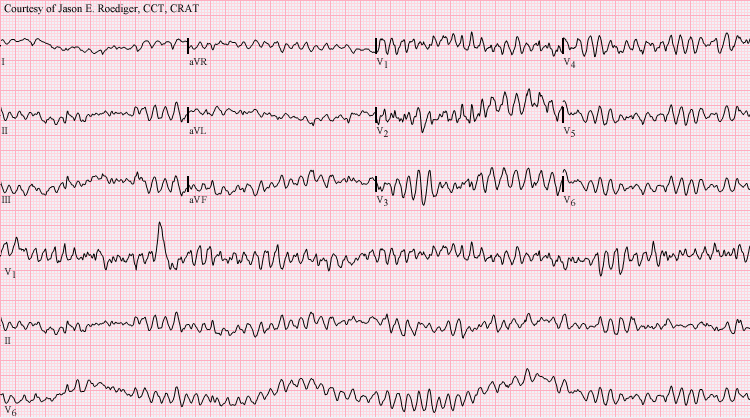
\includegraphics[scale=0.3]{Ventricular_fibrillation.png}
		\caption{Κοιλιακή μαρμαρυγή \en \protect\url{en.wikipedia.org}}
	\end{figure}
	
	
	\begin{figure}[h]
		\centering
		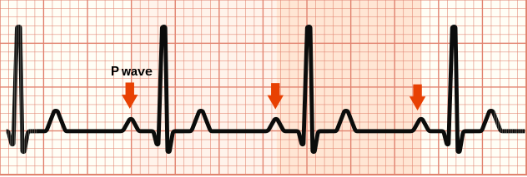
\includegraphics[scale=0.4]{normal.png}
		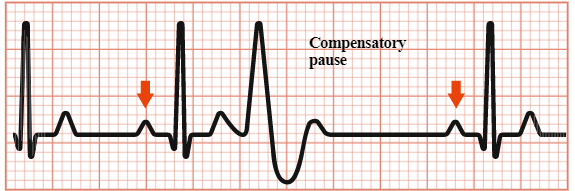
\includegraphics[scale=0.38]{pvc.png}
		\caption{Εκτοπες κοιλιακές συσπάσεις. Στην πρώτη εικόνα (αριστερά) παρουσιάζεται ένας φυσιολογικός καρδιακός ρυθμός και στη δεύτερη (δεξιά) οι έκτοπες κοιλιακές συσπάσεις \en\protect\url{commons.wikimedia.org}}
	\end{figure}
\end{itemize}

\subsubsection{Κομβική αρρυθμία} 
Ο φλεβόκομβος είναι ο βασικός βηματοδότης της καρδιάς και εντοπίζεται στον άνω δεξιό κόλπο της. Ένας δεύτερος βηματοδότης είναι ο κολποκοιλιακός κόμβος και βρίσκεται στον κάτω δεξιό κόλπο. Η δέσμη \en His \gr αποτελεί έναν τρίτο καρδιακό βηματοδότη που βρίσκεται στο όριο ανάμεσα στους κόλπους και τις κοιλίες (συλλογή μυϊκών καρδιακών κυττάρων υπέυθυνων για ηλεκτρικές ώσεις). Ο κομβικός ρυθμός είναι ένας μη φυσιολογικός καρδιακός ρυθμός ο οποίος ξεκινά από τον κολποκοιλιακό κόμβο ή τη δέσμη \en His. \gr Ο ρυθμός αυτός μεταβάλλεται ως εξής: κομβική βραδυκαρδία, όταν ο ρυθμός είναι χαμηλότερος από 40 χτύπους το λεπτό, ρυθμός διαφυγής διασταύρωσης (40-60 παλμούς ανά λεπτό), επιταχυνόμενος κομβικός ρυθμός (60-100 παλμούς ανά λεπτο) και κομβική ταχυκαρδία (περισσότεροι από 100 παλμοί ανά λεπτό). 
\par
Στις περιπτώσεις που η λειτουργία του φλεβόκομβου εμποδίζεται, δημιουργείται ένας κομβικός ρυθμός. Η κατάσταση αυτή μπορεί να προκληθεί από πολυάριθμες καταστάσεις αλλά και φάρμακα. Μερικές τέτοιες καταστάσεις είναι πόνος στο στήθος, ακτινοθεραπεία, μυοκαρδίτιδα, λίθιο, οπιοειδή και κανναβινοειδή.  Τέλος, η αγωγή εξαρτάται κατά κύριο λόγο από τις υποκείμενες αιτίες και νοσήματα.  [42], [43]
‌

\subsubsection{Υπερκοιλιακή αρρυθμία} Ονομάζεται έτσι διότι συμβαίνει στα σημεία άνω του κολποκοιλιακού κόμβου.
\par
Η υπερκοιλιακή αρρυθμία \en (Supraventricular arrhythmia, SVT)\gr προκαλεί στα άτομα που τη βιώνουν έντονη δυσφορία. Μπορεί να εντοπιστεί κατά τη διάρκεια ηλεκτροκαρδιογραφήματος. Η αναλογία ανάμεσα στους άντρες και τις γυναίκες που επηρεάζονται έιναι 1:2 σε όλες τις ηλικίες. Οι βασικές κατηγορίες της είναι η κολποκοιλιακή ταχυκαρδία επανεισόδου, κολποκοιλιακή κομβική ταχυκαρδία επανεισόδου και κολπική ταχυκαρδία, με τη δεύτερη να εμφανίζεται πιο συχνά. Πολύ συχνά, τα επάρματα Ρ δεν είναι εμφανή κατά το ΗΚΓ εξαιτίας της ταυτόχρονης διέγερσης των κόλπων και των κοιλιών και στις περιπτώσεις που διακρίνονται είναι ανεπαίσθητα (ψευδοέπαρμα Ρ). [44]
\par
\textbf{Κολποκοιλιακή κομβική ταχυκαρδία επανεισόδου \en (AVNRT)} \gr \par
\gr Η κολποκοιλιακή κομβική ταχυκαρδία επανεισόδου \en (AVNRT) \gr αποτελεί παροξυσμική υπερκοιλιακή ταχυκαρδία που προκύπτει εξαιτίας κυκλώματος επανεισόδου εντός ή δίπλα στον κολποκοιλιακό κόμβο. Η διάγνωσή της εντοπίζεται κατά τη διάρκεια ΗΚΓ. Στην πλειοψηφία, το ΗΚΓ θα δείξει καρδιακό ρυθμό ανάμεσα σε 140 και 280 παλμών ανά λεπτό και ένα σύμπλεγμα \en QRS \gr μικρότερο από 120 χιλιοστά του δευτερολέπτου. 
\par
Τα συμπτώματα περιλαμβάνουν ζαλάδα, συγκοπή, δύσπνοια, δυσφορία γύρω από το λαιμό και σε άτομα με ιστορικό στεφανιαίας νόσου ακόμα και συμπτώματα εμφράγματος. Η συγκοπή είναι τυπική σε ασθενείς με καρδιακό ρυθμό πάνω από 170 παλμούς το λεπτό, καθώς μικρότερη αιμάτωση των κοιλιών οδηγεί σε μείωση  καρδιακής ικανότητας και μειωμένη αιμάτωση του εγκεφάλου. [35] 
\par

\begin{figure}[h]
	\centering
	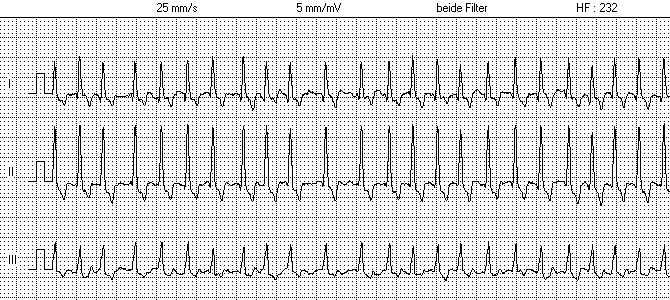
\includegraphics[scale=0.3]{supraventricular tachychardia.jpg}
	\caption{Υπερκοιλιακή ταχυκαρδία \en\protect\url{en.wikipedia.org}}
\end{figure}
\subsection{Με βάση τον καρδιακό ρυθμό}
\subsubsection{Ταχυαρρυθμία η ταχυκαρδία \en (Tachyarrhythmia)} 
Oρίζεται ως αποκλίνων καρδιακός ρυθμός με τουλάχιστον 100 παλμούς το λεπτό. Χωρίζεται με τη σειρά του με βάση το σημείο προέλευσης της αρρυθμίας σε : 

\subsubsection{Βραδυαρρυθμία ή βραδυκαρδία \en (Bradyarrhythmia) \gr}
Κατάσταση κατά την οποία ο καρδιακός ρυθμόε είναι ίσος ή χαμηλότερος των 60 παλμών ανά λεπτό. Συμπεριλαμβάνει διαφορετικές ρυθμικές διαταραχές, οι οποίες παρουσιάζονται στη συνέχεια. Εάν ο ρυθμός μειωθεί σε μεγάλο βαθμό, η παροχή αίματος στον εγκέφαλο περιορίζεται με αποτέλεσμα τη λιποθυμία.
\par
Ο φλεβόκομβος είναι βασικός βηματοδότης της καρδιάς, αποκτώντας με αυτό τον τρόπο σημαντικό ρόλο στην κυκλοφορία του αίματος και τη λειτουργία του μυοκαρδίου. Η φλεβοκομβική βραδυκαρδία αποτελεί ένα καρδιακό ρυθμό κατά τον οποίο αν και οι παλμοί είναι χαμηλότεροι του φυσιολογικού δεν υπάρχει κάποια δομική αδυναμία ή ανωμαλία. Μπορεί να διαγνωστεί μέσω ΗΚΓ και η απεικόνιση είναι αυτή ενός φυσιολογικού καρδιακού ρυθμού σε μορφολογία αν και είναι χαμηλότερος. Εμφανίζεται κυρίως σε άτομα άνω των 65 και σε νεόυς αθλητές.
\par
Οι αιτίες της βραδυκαρδίας είναι τόσο εσωτερικές όσο και εξωτερικές. Οι εσωτερικές μπορεί να είναι τραύμα στο στήθος, έμφραγμα του μυοκαρδίου, στεφανιαία νόσος, μυοκαρδίτιδα, νόσος του \en Lyme \gr και πολλές ακόμα. Κύριες εξωγενείς αιτίες αποτελούν κυρίως φαρμακευτικές αγωγές όπως οι β-αναστολείς και στη συνέχεια η χρήση ναρκωτικών ουσιών και τα κανναβινοειδή, ο υποθυρεοειδισμός, η άπνοια, ακόμα και η νευρική ανορεξία. 
\par
\begin{figure}
	\centering
	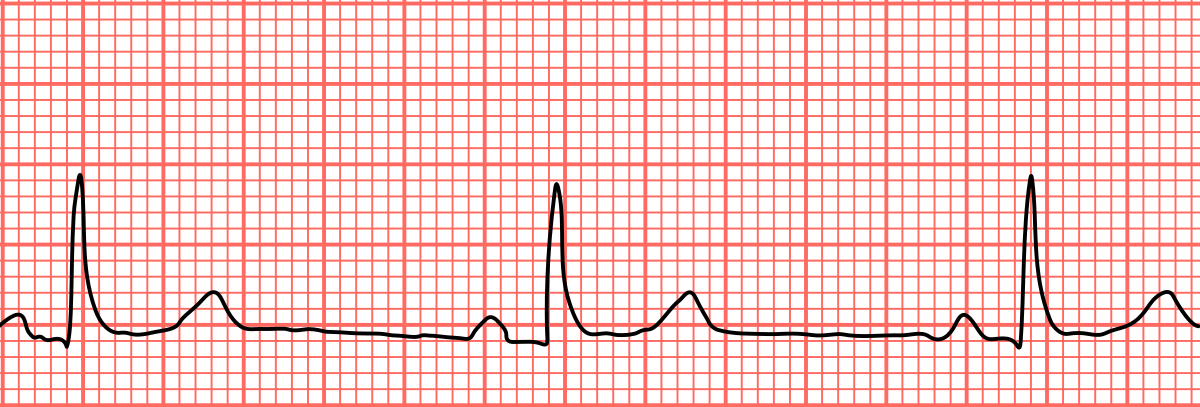
\includegraphics[scale=0.2]{bradychardia.png}
	\caption{Βραδυκαρδία \en\protect\url{en.wikipedia.org}}
\end{figure}
Η πλειοψηφία των ασθενών με βραδυκαρδία δεν παρουσιάζουν κάποια συμπτώματα. Υγιείς ενήλικες νεαρής ηλικίας και αθλητές σε κατάσταση ηρεμίας εμφανίζουν βραδυκαρδία λόγω του αυξημένου πνευμονογαστρικού τόνου (\en increased vagal tone),\gr γεγονός που δηλώνει αυκημένη καρδιακή μεταβλητότητα. Βραδυκαρδία εμφανίζεται και σε ενήλικες άνω των 65 σε κατάσταση ύπνου, που οφείλεται στη γήρανση του φλεβόκομβου [18]-[26], [40], [41]. 
\par

%\end{document}
